% Asset ID: FAS2AlgorithmsOnGraphsTikZ-002
% Source: Supplied PDF Dijkstra's algorithm notation and worked example
% Related lesson section: Section 9 Visual Asset Integration
% Purpose: Show Dijkstra label-box structure and a worked shortest-path network.
\documentclass[tikz,border=8pt]{standalone}
\usepackage{xcolor}
\usepackage{tikz}
\usetikzlibrary{positioning,calc}
\definecolor{canvas}{HTML}{FAF9F6}
\definecolor{panel}{HTML}{FFFFF0}
\definecolor{line}{HTML}{E5E5EA}
\definecolor{accent}{HTML}{C5A059}
\definecolor{textcol}{HTML}{2C2C2E}
\definecolor{muted}{HTML}{9A9AA0}
\begin{document}
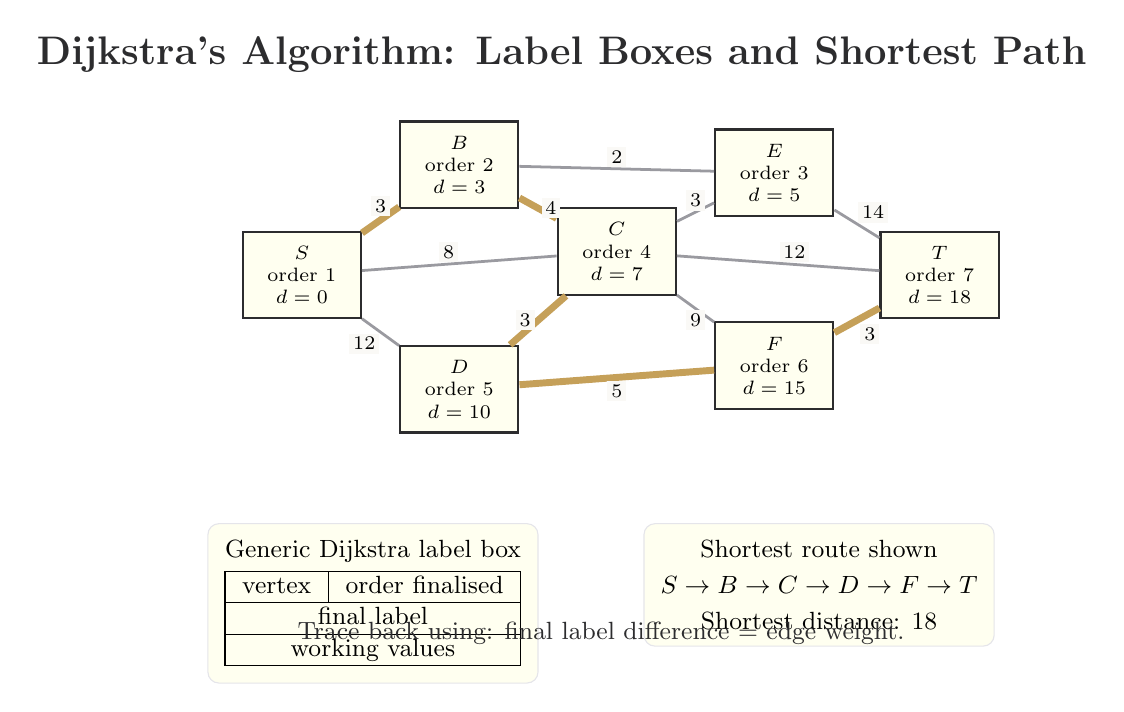
\begin{tikzpicture}[
    vertexbox/.style={draw=textcol,fill=panel,line width=0.8pt,minimum width=15mm,minimum height=11mm,align=center,font=\scriptsize},
    pathEdge/.style={draw=accent,line width=2.5pt},
    otherEdge/.style={draw=muted,line width=1.0pt},
    weight/.style={fill=canvas,inner sep=1.4pt,font=\scriptsize},
    note/.style={draw=line,fill=panel,rounded corners=4pt,inner sep=6pt,align=center,font=\small},
    title/.style={align=center,font=\Large\bfseries,text=textcol}
]
\node[title] at (3.3,4.5) {Dijkstra's Algorithm: Label Boxes and Shortest Path};
\node[vertexbox] (S) at (0,1.7) {$S$\\order $1$\\$d=0$};
\node[vertexbox] (B) at (2.0,3.1) {$B$\\order $2$\\$d=3$};
\node[vertexbox] (C) at (4.0,2.0) {$C$\\order $4$\\$d=7$};
\node[vertexbox] (D) at (2.0,0.25) {$D$\\order $5$\\$d=10$};
\node[vertexbox] (E) at (6.0,3.0) {$E$\\order $3$\\$d=5$};
\node[vertexbox] (F) at (6.0,0.55) {$F$\\order $6$\\$d=15$};
\node[vertexbox] (T) at (8.1,1.7) {$T$\\order $7$\\$d=18$};
\draw[otherEdge] (S) -- node[weight,above left] {$8$} (C);
\draw[otherEdge] (S) -- node[weight,below left] {$12$} (D);
\draw[otherEdge] (B) -- node[weight,above] {$2$} (E);
\draw[otherEdge] (C) -- node[weight,above] {$3$} (E);
\draw[otherEdge] (C) -- node[weight,below] {$9$} (F);
\draw[otherEdge] (C) -- node[weight,above right] {$12$} (T);
\draw[otherEdge] (E) -- node[weight,above right] {$14$} (T);
\draw[pathEdge] (S) -- node[weight,above] {$3$} (B);
\draw[pathEdge] (B) -- node[weight,right] {$4$} (C);
\draw[pathEdge] (C) -- node[weight,left] {$3$} (D);
\draw[pathEdge] (D) -- node[weight,below] {$5$} (F);
\draw[pathEdge] (F) -- node[weight,below right] {$3$} (T);
\node[note,anchor=north west] at (-1.2,-1.45) {Generic Dijkstra label box\\[2pt]\begin{tabular}{|c|c|}\hline vertex & order finalised\\\hline \multicolumn{2}{|c|}{final label}\\\hline \multicolumn{2}{|c|}{working values}\\\hline\end{tabular}};
\node[note,anchor=north east] at (8.8,-1.45) {Shortest route shown\\[2pt]$S \to B \to C \to D \to F \to T$\\[2pt]Shortest distance: $18$};
\node[align=center,font=\small,text=textcol] at (3.8,-2.85) {Trace back using: final label difference $=$ edge weight.};
\end{tikzpicture}
\end{document}
